\documentclass[11pt, spanish]{report}

%Needed to use diagbox that make the \ in the table
\usepackage{diagbox}
%Needed to insert any photo
\usepackage{graphicx}
%Needed to insert links
\usepackage{hyperref}


\usepackage[a4paper, total={6.5in, 8in}]{geometry}

\usepackage{graphicx}
\graphicspath{ {images/} }

\usepackage[spanish]{babel}
\usepackage{circuitikz}
\selectlanguage{spanish}
\usepackage[utf8]{inputenc}

%\documentclass{report} %Usar REPORT para que reconozca CHAPTERS!
\usepackage{amsmath}
\usepackage{tikz}
\usetikzlibrary{matrix,calc}
\usepackage{tikz}

%isolated term
%#1 - Optional. Space between node and grouping line. Default=0
%#2 - node
%#3 - filling color
\newcommand{\implicantsol}[3][0]{
    \draw[rounded corners=3pt, fill=#3, opacity=0.3] ($(#2.north west)+(135:#1)$) rectangle ($(#2.south east)+(-45:#1)$);
    }


%internal group
%#1 - Optional. Space between node and grouping line. Default=0
%#2 - top left node
%#3 - bottom right node
%#4 - filling color
\newcommand{\implicant}[4][0]{
    \draw[rounded corners=3pt, fill=#4, opacity=0.3] ($(#2.north west)+(135:#1)$) rectangle ($(#3.south east)+(-45:#1)$);
    }

%group lateral borders
%#1 - Optional. Space between node and grouping line. Default=0
%#2 - top left node
%#3 - bottom right node
%#4 - filling color
\newcommand{\implicantcostats}[4][0]{
    \draw[rounded corners=3pt, fill=#4, opacity=0.3] ($(rf.east |- #2.north)+(90:#1)$)-| ($(#2.east)+(0:#1)$) |- ($(rf.east |- #3.south)+(-90:#1)$);
    \draw[rounded corners=3pt, fill=#4, opacity=0.3] ($(cf.west |- #2.north)+(90:#1)$) -| ($(#3.west)+(180:#1)$) |- ($(cf.west |- #3.south)+(-90:#1)$);
}

%group top-bottom borders
%#1 - Optional. Space between node and grouping line. Default=0
%#2 - top left node
%#3 - bottom right node
%#4 - filling color
\newcommand{\implicantdaltbaix}[4][0]{
    \draw[rounded corners=3pt, fill=#4, opacity=0.3] ($(cf.south -| #2.west)+(180:#1)$) |- ($(#2.south)+(-90:#1)$) -| ($(cf.south -| #3.east)+(0:#1)$);
    \draw[rounded corners=3pt, fill=#4, opacity=0.3] ($(rf.north -| #2.west)+(180:#1)$) |- ($(#3.north)+(90:#1)$) -| ($(rf.north -| #3.east)+(0:#1)$);
}

%group corners
%#1 - Optional. Space between node and grouping line. Default=0
%#2 - filling color
\newcommand{\implicantcantons}[2][0]{
    \draw[rounded corners=3pt, opacity=.3] ($(rf.east |- 0.south)+(-90:#1)$) -| ($(0.east |- cf.south)+(0:#1)$);
    \draw[rounded corners=3pt, opacity=.3] ($(rf.east |- 8.north)+(90:#1)$) -| ($(8.east |- rf.north)+(0:#1)$);
    \draw[rounded corners=3pt, opacity=.3] ($(cf.west |- 2.south)+(-90:#1)$) -| ($(2.west |- cf.south)+(180:#1)$);
    \draw[rounded corners=3pt, opacity=.3] ($(cf.west |- 10.north)+(90:#1)$) -| ($(10.west |- rf.north)+(180:#1)$);
    \fill[rounded corners=3pt, fill=#2, opacity=.3] ($(rf.east |- 0.south)+(-90:#1)$) -|  ($(0.east |- cf.south)+(0:#1)$) [sharp corners] ($(rf.east |- 0.south)+(-90:#1)$) |-  ($(0.east |- cf.south)+(0:#1)$) ;
    \fill[rounded corners=3pt, fill=#2, opacity=.3] ($(rf.east |- 8.north)+(90:#1)$) -| ($(8.east |- rf.north)+(0:#1)$) [sharp corners] ($(rf.east |- 8.north)+(90:#1)$) |- ($(8.east |- rf.north)+(0:#1)$) ;
    \fill[rounded corners=3pt, fill=#2, opacity=.3] ($(cf.west |- 2.south)+(-90:#1)$) -| ($(2.west |- cf.south)+(180:#1)$) [sharp corners]($(cf.west |- 2.south)+(-90:#1)$) |- ($(2.west |- cf.south)+(180:#1)$) ;
    \fill[rounded corners=3pt, fill=#2, opacity=.3] ($(cf.west |- 10.north)+(90:#1)$) -| ($(10.west |- rf.north)+(180:#1)$) [sharp corners] ($(cf.west |- 10.north)+(90:#1)$) |- ($(10.west |- rf.north)+(180:#1)$) ;
}

%Empty Karnaugh map 4x4
\newenvironment{Karnaugh}%
{
\begin{tikzpicture}[baseline=(current bounding box.north),scale=0.8]
\draw (0,0) grid (4,4);
\draw (0,4) -- node [pos=0.7,above right,anchor=south west] {cd} node [pos=0.7,below left,anchor=north east] {ab} ++(135:1);
%
\matrix (mapa) [matrix of nodes,
        column sep={0.8cm,between origins},
        row sep={0.8cm,between origins},
        every node/.style={minimum size=0.3mm},
        anchor=8.center,
        ampersand replacement=\&] at (0.5,0.5)
{
                       \& |(c00)| 00         \& |(c01)| 01         \& |(c11)| 11         \& |(c10)| 10         \& |(cf)| \phantom{00} \\
|(r00)| 00             \& |(0)|  \phantom{0} \& |(1)|  \phantom{0} \& |(3)|  \phantom{0} \& |(2)|  \phantom{0} \&                     \\
|(r01)| 01             \& |(4)|  \phantom{0} \& |(5)|  \phantom{0} \& |(7)|  \phantom{0} \& |(6)|  \phantom{0} \&                     \\
|(r11)| 11             \& |(12)| \phantom{0} \& |(13)| \phantom{0} \& |(15)| \phantom{0} \& |(14)| \phantom{0} \&                     \\
|(r10)| 10             \& |(8)|  \phantom{0} \& |(9)|  \phantom{0} \& |(11)| \phantom{0} \& |(10)| \phantom{0} \&                     \\
|(rf) | \phantom{00}   \&                    \&                    \&                    \&                    \&                     \\
};
}%
{
\end{tikzpicture}
}

%Empty Karnaugh map 2x4
\newenvironment{Karnaughvuit}%
{
\begin{tikzpicture}[baseline=(current bounding box.north),scale=0.8]
\draw (0,0) grid (4,2);
\draw (0,2) -- node [pos=0.7,above right,anchor=south west] {bc} node [pos=0.7,below left,anchor=north east] {a} ++(135:1);
%
\matrix (mapa) [matrix of nodes,
        column sep={0.8cm,between origins},
        row sep={0.8cm,between origins},
        every node/.style={minimum size=0.3mm},
        anchor=4.center,
        ampersand replacement=\&] at (0.5,0.5)
{
                      \& |(c00)| 00         \& |(c01)| 01         \& |(c11)| 11         \& |(c10)| 10         \& |(cf)| \phantom{00} \\
|(r00)| 0             \& |(0)|  \phantom{0} \& |(1)|  \phantom{0} \& |(3)|  \phantom{0} \& |(2)|  \phantom{0} \&                     \\
|(r01)| 1             \& |(4)|  \phantom{0} \& |(5)|  \phantom{0} \& |(7)|  \phantom{0} \& |(6)|  \phantom{0} \&                     \\
|(rf) | \phantom{00}  \&                    \&                    \&                    \&                    \&                     \\
};
}%
{
\end{tikzpicture}
}

%Empty Karnaugh map 2x2
\newenvironment{Karnaughquatre}%
{
\begin{tikzpicture}[baseline=(current bounding box.north),scale=0.8]
\draw (0,0) grid (2,2);
\draw (0,2) -- node [pos=0.7,above right,anchor=south west] {b} node [pos=0.7,below left,anchor=north east] {a} ++(135:1);
%
\matrix (mapa) [matrix of nodes,
        column sep={0.8cm,between origins},
        row sep={0.8cm,between origins},
        every node/.style={minimum size=0.3mm},
        anchor=2.center,
        ampersand replacement=\&] at (0.5,0.5)
{
          \& |(c00)| 0          \& |(c01)| 1  \\
|(r00)| 0 \& |(0)|  \phantom{0} \& |(1)|  \phantom{0} \\
|(r01)| 1 \& |(2)|  \phantom{0} \& |(3)|  \phantom{0} \\
};
}%
{
\end{tikzpicture}
}

%Defines 8 or 16 values (0,1,X)
\newcommand{\contingut}[1]{%
\foreach \x [count=\xi from 0]  in {#1}
     \path (\xi) node {\x};
}

%Places 1 in listed positions
\newcommand{\minterms}[1]{%
    \foreach \x in {#1}
        \path (\x) node {1};
}

%Places 0 in listed positions
\newcommand{\maxterms}[1]{%
    \foreach \x in {#1}
        \path (\x) node {0};
}

%Places X in listed positions
\newcommand{\indeterminats}[1]{%
    \foreach \x in {#1}
        \path (\x) node {X};
}
\begin{document}
\title{Electronica III \\
Trabajo Practico de Laboratorio N 1}

\author{Martin Rodriguez Turco\\
 Juan Martin Laguinge\\
 Tobias Scala\\
 Guido Panaggio}
\date{5 de Septiembre de 2018}

\begin{Large}
\maketitle
\end{Large}

%\documentclass[11pt]{article}

%\begin{document}
\chapter*{1-Rango y Resoluci\'on}

\section{Objetivo}
\indent\indent  Desarrollar un programa que calcule el Rango y Resoluci\'on de un n\'umero de punto fijo.\\
\indent El mismo recibira el signo, cantidad de bits de la parte entera y la cantidad de bits de la parte fraccionaria.
\section{Calculo de Rango y Observaciones}
\indent\indent Para poder hacer el calculo del Rango se deben tomar en cuenta los 3 parametros mencionados. Esto se debe a que se debe distinguir si el n\' umero es de tipo signado (SIGNO = 1) o no (SIGNO = 0). Esto parece ser estrictamente necesario. Sin embargo m\'as adelante veremos que no lo es.
\\ \indent Comenzamos por enunciar la definici\'on de Rango:\\
	\begin{center}
	\emph{Es la diferencia entre la magnitud representable m\'as positiva y la magnitud representable m\'as negativa}
	\end{center}

\subsection{Ejemplo de c\'alculo de Rango}
\indent\indent Introduciremos el metodo de c\'alculo mediante un ejemplo:\\
\indent Supongamos que deseamos calcular el rango \textbf{R} de un n\'umero binario \textit{signado} con $3\ bits$ de parte entera y $2\ bits$ de parte fraccionaria entonces tenemos un n\'umero con la siguiente forma:



\begin{center}
\begin{tabular}{ |c|c|c|c|c| } 
 \hline
 2 & 1 & 0 & -1 & -2 \\ 
 x & x & x  & x & x\\ 
 \hline
\end{tabular}
\end{center}

Para calcular el maximo n\'umero representable $M$ :
\begin{center}
\begin{tabular}{ |ccccc| } 
 \hline
 0 & 1 & 1 & .1 & 1 \\ 
 \hline
\end{tabular}
\end{center}
$$ 0^2 + 2^1 + 2^0 +2^{-1} + 2^{-2}  = 3.75$$
\\\\
Para calcular el minimo n\'umero representable $m$ :
\begin{center}

\begin{tabular}{ |ccccc| } 
 \hline
 1 & 0 & 0 & .0 & 0 \\ 
 \hline
\end{tabular}
\end{center}
$$ m = -2^{2} = -4$$

Por lo tanto el rango: 
$$R = 3.75 - (-4 )$$ 
$$R = 7.75 $$
\\
\indent Ahora podemos preguntarnos  C\'omo realizar el c\'alculo s\'i el n\'umero es no \textit{signado}.
\\\\
La maxima denominaci\'on vendra dada por:
\begin{center}
\begin{tabular}{ |ccccc| } 
 \hline
 1 & 1 & 1 & .1 & 1 \\ 
 \hline
\end{tabular}
\end{center}

$$M' = 2^2 + 2^1 + 2^0 + 2^{-1} + 2^{-2}$$
$$M' = 7.75$$
\\
La minima denominaci\'on vendra dada por:
\begin{center}
\begin{tabular}{ |ccccc| } 
 \hline
 0 & 0 & 0 & .0 & 0 \\ 
 \hline
\end{tabular}
\end{center}

Lo cual claramente indicia que el minimo n\'umero representable es el $0$. Por lo tanto: $$m = 0$$




Entonces: 	$$R' = M' - m'$$
		 	$$R' = 7.75 $$
		 	
		 	
Notamos que $R = R'$. Esto nos da indicios de que el rango de un n\'umero de punto fijo \textit{signado} \'o \textit{no signado} tiene n el mismo rango. A continuaci\'on demostraremos que esto es de hecho as\'i.

\subsection{Formula general para el c\'alculo del Rango}



 
%\end{document}



\chapter*{2-Mapas de Karnaugh y Algebra de Boole}
\section{Objetivo}
\indent\indent Obtener la representación en mapas de Karnaugh de una función dada. Esta misma debera ser simplifacada aplicando las tecnicas de agrupación vistas en clase. Además se debera realizar mediante el método tradicional del Algebra de Boole.

Finalmente modelaremos el sistema resultante con su correspondiente circuito logico. Luego, dado se expresara este mismo haciendo uso unicamente de compuertas \textit{nand}.

\subsection{Obtención del mapa de Karnaugh}
Dada la siguiente expresión en maxtérminos se pudo interpretar el mapa de Karnaugh de donde provinieron
\[
	f(a,b,c,d)=\prod\left(M_{0},M_{1},M_{5},M_{7},M_{8},M_{10},M_{14},M_{15}\right)
\]
\begin{center}
 \begin{Karnaugh}
 %Inputs are in the order of the max/min termns. Do not use continous inputs. Ex: first term refers to m0/M0, fourth term refers to m2/M2
        \contingut{0,0,1,1,1,0,1,0,0,1,0,1,1,1,0,0}
       	\implicant{2}{6}{red}
       	\implicant{13}{9}{blue}	%Numero de mintermino o Maxtermino
     	\implicant{4}{12}{purple}
     	\implicantdaltbaix[3pt]{3}{11}{green}
    %\implicantcantons[2pt]{orange}
      	%\implicantcostats{3}{11}{green}
    \end{Karnaugh}
\end{center}

Mediante la selección de dichos grupos se obtuvo la siguiente función logica simplificada mediante mintérminos:
\[
	f(a,b,c,d)= b\overline{cd} + a\overline{c}d +
				\overline{b}cd +\overline{a}c\overline{d}
\]

Dado que se han escogido 4 grupos se ha llegado de forma inmediata a dicha formulación

\subsection{Aplicaci\'on del algebra de Boole}
\indent En este apartado desarrollaremos paso por paso las operaciones necesarias para obtener la expresión logica simplificada del sistema dado.
\indent 
Nuestro primer paso es plantear la suma de de los mintérminos:
\[f(a,b,c,d)= \underbrace{\overline{ab}cd}_{m_3}+
			  \underbrace{\overline{ab}c\overline{d}}_{m_2}
			 +\underbrace{\overline{a}b\overline{cd}}_{m_4}
			 +\underbrace{\overline{a}bc\overline{d}}_{m_6}
			 +\underbrace{ab\overline{cd}}_{m_{12}}
			 +\underbrace{ab\overline{c}d}_{m_{13}}
			 +\underbrace{a\overline{bc}d}_{m_9} 
			 +\underbrace{a\overline{b}cd}_{m_{11}}
			 \]
El resultado de su simplificación dependera de cómo se sumen los terminos. 
Primero aplicaremos ciegamente las reglas de simplificación:
\[ 
	f(a,b,c,d)= \underbrace{\overline{ab}c\underbrace{\left(d+ \overline{d}\right)}_{1}}_{m_3 +m_2}
	+
	\underbrace{\overline{a}b\overline{d}\underbrace{\left(c+ \overline{c}\right)}_{1}}_{m_4 +m_6}
	+
	\underbrace{ab\overline{c}\underbrace{\left(d+ \overline{d}\right)}_{1}}_{m_{12} +m_{13}}
	+
	\underbrace{a\overline{b}d\underbrace{\left(c+ \overline{c}\right)}_{1}}_{m_9 +m_{11}}
\]

La expresión simplificada:
\[ 
	f(a,b,c,d)= 
	\overline{ab}c
	+
	\overline{a}b\overline{d}
	+
	ab\overline{c}
	+
	a\overline{b}d
\]


Esta expresión tiene la misma cantidad de terminos que la obtenida mediane el mapa de Karnaugh. 
Ahora se realizara de nuevo la suma pero esta vez se agruparan tal como fueron escogidos los grupos en el mapa.

$$
f(a,b,c,d)= 
\underbrace{\overline{ab}cd + a\overline{b}cd}_{m_3 + m_{11}}
+
\underbrace{\overline{a}b\overline{cd} + ab\overline{cd}}_{m_4+m_{12}}
+
\underbrace{ab\overline{c}d + a\overline{bc}d }_{m_{13} + m_{9}}
+
\underbrace{\overline{ab}c\overline{d} + \overline{a}bc\overline{d}}_{m_2 + m_6}
$$

Simplificando:
$$f(a,b,c,d)= 
\underbrace{\overline{b}cd\underbrace{\left(\overline{a}+a\right)}_{1}}_{m_3 + m_{11}}
+\underbrace{b\overline{cd}\underbrace{\left(\overline{a}+a\right)}_{1}}_{m_4+m_{12}}
+
\underbrace{a\overline{c}d\underbrace{\left(\overline{c}+c\right)}_{1} }_{m_{13} + m_{9}}
+
\underbrace{\overline{a}b\overline{d}\underbrace{\left(\overline{b}+b\right)}_{1}}_{m_2 + m_6}$$


Finalmente, reacomodando los terminos:
\[
	f(a,b,c,d)= b\overline{cd} + a\overline{c}d +
				\overline{b}cd +\overline{a}c\overline{d}
\]

Llegamos nuevamente a la expresión deducida mediane el mapa de 
Karnaugh

\section{Circuito Logico}




\chapter*{3-Encoder y Demux}
\section{Encoder}
%\indent
\subsection{Objetivo}
Desarrollar un m\'odulo en Verilog el cual funcione como un encoder de 4 entradas.
\subsection{Explicaci\'on y Desarrollo}
Un encoder tiene la funcionalidad de tomar los datos de entrada y los codifica para que las salidas
representen (en n\'umero en binario) la entrada cuyo valor es 1 como se puede ver en la siguiente tabla de verdad.
\begin{center}
	\begin{table}[h!]
		\begin{center}
			\caption{Tabla de Verdad del Encoder}
			\begin{tabular}{|c|c|}
				\hline
				\textbf{INPUT} & \textbf{OUTPUT} \\
				\hline
				\textbf{a b c d} & \textbf{x y} \\
				\hline
				0 0 0 0 & z z\\
				\hline
				0 0 0 1 & 0 0 \\
				\hline
				0 0 1 0 & 0 1\\
				\hline
				0 0 1 1 & z z\\
				\hline
				0 1 0 0 & 1 0\\
				\hline
				0 1 0 1 & z z\\
				\hline
				0 1 1 0 & z z\\
				\hline
				0 1 1 1 & z z\\
				\hline
				1 0 0 0 & 1 1\\
				\hline
				1 0 0 1 & z z\\
				\hline
				1 0 1 0 & z z\\
				\hline
				1 0 1 1 & z z\\
				\hline
				1 1 0 0 & z z\\
				\hline
				1 1 0 1 & z z\\
				\hline
				1 1 1 0 & z z\\
				\hline
				1 1 1 1 & z z\\
				\hline
			\end{tabular} \\
		\end{center}
	\end{table}
\end{center}
Como las \'unicas salidas v\'alidas del encoder son aquellas cuando hay una \'unica entrada que contiene un 1, las dem\'as combinaciones de entradas se consideran como comodines para las salidas. Las cuales
se puede elegir su valor de tal forma de facilitar los cálculos para obtener la funci\'on l\'ogica.
Para poder obtener la fuci\'on l\'ogica del mismo, se hizo uso del mapa de Karnaugh el cual se muestra
a continuación.
\\
\begin{Karnaugh}
	%\caption{Tabla de Verdad del Encoder}
    \contingut{z,1,1,z,0,z,z,z,0,z,z,z,z,z,z,z}
    %\implicant{0}{2}{red}
    %\implicant{5}{15}{purple}
    %\implicantdaltbaix[3pt]{3}{10}{blue}
    %\implicantcantons[2pt]{orange}
    %\implicantcostats{4}{14}{green}
\end{Karnaugh}
\begin{Karnaugh}
	%\caption{Tabla de Verdad del Encoder}
    \contingut{z,0,1,z,0,z,z,z,1,z,z,z,z,z,z,z}
    %\implicant{0}{2}{red}
    %\implicant{5}{15}{purple}
    %\implicantdaltbaix[3pt]{3}{10}{blue}
    %\implicantcantons[2pt]{orange}
    %\implicantcostats{4}{14}{green}
\end{Karnaugh}
\\
El mapa de Karnaugh de la izquierda corresponde la salida X y el de la derecha la salida Y.
Empezando con el mapa correspondiente a la salida X, se eligieron los valores de los comodines (z) de forma conveniente para poder agrupar lo m\'as posible. Este mapa se lo resolver\'a utilizando mint\'erminos.

\begin{center}
\begin{Karnaugh}
    \contingut{1,1,1,1,0,0,1,1,0,0,1,1,0,0,1,1}
    \implicant{3}{10}{red}
    \implicant{0}{2}{blue}
\end{Karnaugh}
\end{center}

Ahora, para poder armar la funci\'on l\'ogica, se debe ver qu\'e variable (dentro de cada grupo) no cambia su valor. Y si dicha variable contiene el valor 0, entonces se lo niega ya que estamos trabajando con mint\'erminos. Se obtiene la siguiente funci\'on l\'ogica para la salida X.

\begin{center}
X = Not(c)Not(d) + a
\end{center}
Cuya tabla de verdad se muestra a continuación.
\begin{center}
	\begin{table}[h!]
		\begin{center}
			\caption{Tabla de Verdad del Encoder}
			\begin{tabular}{|c|c|}
				\hline
				\textbf{INPUT} & \textbf{OUTPUT} \\
				\hline
				\textbf{a c d} & \textbf{x} \\
				\hline
				0 0 0 & 1\\
				\hline
				0 0 1 & 1 \\
				\hline
				0 1 0 & 0\\
				\hline
				0 1 1 & 1\\
				\hline
				1 0 0 & 0\\
				\hline
				1 0 1 & 1\\
				\hline
				1 1 0 & 0\\
				\hline
				1 1 1 & 1\\
				\hline
			\end{tabular} \\
		\end{center}
	\end{table}
\end{center}

Ahora centr\'andose en el mapa correspondiente a la salida Y, se eligieron nuevamente los valores de los comodines (z) de forma conveniente para poder agrupar lo m\'as posible. Este mapa se lo resolver\'a utilizando maxt\'erminos.

\begin{center}
\begin{Karnaugh}
    \contingut{0,0,1,1,0,0,1,1,1,1,0,0,1,1,0,0}
    \implicant{0}{5}{red}
    \implicant{15}{10}{blue}
\end{Karnaugh}
\end{center}

Para poder armar la funci\'on l\'ogica, se debe ver nuevamente qu\'e variable (dentro de cada grupo) no cambia su valor. Y si dicha variable contiene el valor 1, entonces se lo niega ya que estamos trabajando con maxt\'erminos. Se obtiene la siguiente funci\'on l\'ogica para la salida Y.

\begin{center}
$$Y = a\overline{c} + c\overline{a}$$
\end{center}
Cuya tabla de verdad se muestra a continuaci\'on.
\begin{center}
	\begin{table}[h!]
		\begin{center}
			\caption{Tabla de Verdad del Encoder}
			\begin{tabular}{|c|c|}
				\hline
				\textbf{INPUT} & \textbf{OUTPUT} \\
				\hline
				\textbf{a c} & \textbf{y} \\
				\hline
				0 0 & 0\\
				\hline
				0 1 & 1 \\
				\hline
				1 0 & 1\\
				\hline
				1 1 & 0\\
				\hline
			\end{tabular} \\
		\end{center}
	\end{table}
\end{center}
Se puede notar, a trav\'es de la tabla de verdad, que $$Y = xor(a,c)$$
\section{Demux}
\subsection{Objectivo}
Desarrollaar un módulo en Verilog el cual implemente el concepto de Demux.

\subsection{Criterio e implementación}
Dado que un componenete del tipo Demux tiene por finalidad dirigir su entrada hacia una salida en particular se realizo la siguiente observación:
\begin{center}
\textit{Si la entrada es nula su salida sera nula en todas las terminales}
\end{center}
Teniendo dicho conocimiento podemos evitar realizar cualquier tipo de calculo dado que al conocer la entrada la salida queda completamente determinada.
No es así en el caso de que la entrada sea 1 dado que cualquiera de los 4 terminales de salida puede ser esocgido para reflejar el valor de entrada.
Para su implementación en Verilog se decidio implementar mediante shifteos de 1 bit. Es decir que para evitar definir la solución de manera anticipada (dado que desconocemos las consecuencias de su implementación en la vida real). En otras palabra, definir una constante puede incurrir en un gasto de energía constante mientras que la realización de un calculo cuando es necesario puede ser beneficioso.



\chapter*{Ejercicio 4}

Para lograr ver los mintérminos que poseen los bits de salida realizamos la siguinte tabla de verdad:
\begin{center}
	\begin{table}[h!]
		\begin{center}
			\caption{Tabla de Verdad}
			\begin{tabular}{|c|c|}
				\hline
				\textbf{INPUT} & \textbf{OUTPUT} \\
				\hline
				0 0 0 0 & 0 0 0 0\\
				\hline
				0 0 0 1 & 1 1 1 1\\
				\hline
				0 0 1 0 & 1 1 1 0\\
				\hline
				0 0 1 1 & 1 1 0 1\\
				\hline
				0 1 0 0 & 1 1 0 0\\
				\hline
				0 1 0 1 & 1 0 1 1\\
				\hline
				0 1 1 0 & 1 0 1 0\\
				\hline
				0 1 1 1 & 1 0 0 1\\
				\hline
				1 0 0 0 & 1 0 0 0\\
				\hline
				1 0 0 1 & 0 1 1 1\\
				\hline
				1 0 1 0 & 0 1 1 0\\
				\hline
				1 0 1 1 & 0 1 0 1\\
				\hline
				1 1 0 0 & 0 1 0 0\\
				\hline
				1 1 0 1 & 0 0 1 1\\
				\hline
				1 1 1 0 & 0 0 1 0\\
				\hline
				1 1 1 1 & 0 0 0 1\\
				\hline
			\end{tabular} \\
		\end{center}
	\end{table}
\end{center}
Siendo X el primer bit de la izquierda,Y el segundo, W el tercero y Z el ultimo del OUTPUT; y  siendo A el primer bit de la izquierda,B el segundo,C el tercero y D el ultimo. Obtenemos las siguentes salidas dadas en funcion de los minterminos:
	$$ X= m1+m2+m3+m4+m5+m6+m7+m8$$ 
	$$ Y = m1+m2+m3+m4+m9+m10+m11+m12$$
	$$ W = m1+m2+m5+m6+m9+m10+m13+m14$$
	$$ Z = m1+m3+m5+m7+m9+m11+m13+m15$$
Reemplazando los minterminos mi por sus respectivos valores nos queda la siguiente repuesta:
	\begin{center}
		$$ X =  \overline{A} \cdot \overline{B} \cdot \overline{C} \cdot D  +  \overline{A} \cdot \overline{B} \cdot C \cdot \overline{D} + \overline{A} \cdot \overline{B} \cdot C \cdot D + \overline{A} \cdot B \cdot \overline{C} \cdot \overline{D} + \overline{A} \cdot B \cdot \overline{C} \cdot D + \overline{A} \cdot B \cdot C \cdot \overline{D} + \overline{A} \cdot B \cdot C \cdot D+  A \cdot \overline{B} \cdot \overline{C} \cdot \overline{D} $$
$$ Y =  \overline{A} \cdot \overline{B} \cdot \overline{C} \cdot D  +  \overline{A} \cdot \overline{B} \cdot C \cdot \overline{D} + \overline{A} \cdot \overline{B} \cdot C \cdot D + \overline{A} \cdot B \cdot \overline{C} \cdot \overline{D} + A \cdot \overline{B} \cdot \overline{C} \cdot D + A \cdot \overline{B} \cdot C \cdot \overline{D} + A \cdot \overline{B} \cdot C \cdot D+  A \cdot B \cdot \overline{C} \cdot \overline{D} $$
$$ W =  \overline{A} \cdot \overline{B} \cdot \overline{C} \cdot D  +  \overline{A} \cdot \overline{B} \cdot C \cdot \overline{D} + \overline{A} \cdot B \cdot \overline{C} \cdot D + \overline{A} \cdot B \cdot C \cdot \overline{D} + A \cdot \overline{B} \cdot \overline{C} \cdot D + A \cdot \overline{B} \cdot C \cdot \overline{D} + A \cdot B \cdot \overline{C} \cdot D+  A \cdot B \cdot C \cdot \overline{D} $$
$$ Z =  \overline{A} \cdot \overline{B} \cdot \overline{C} \cdot D  +  \overline{A} \cdot \overline{B} \cdot C \cdot D + \overline{A} \cdot B \cdot \overline{C} \cdot D + \overline{A} \cdot B \cdot C \cdot D + A \cdot \overline{B} \cdot \overline{C} \cdot D + A \cdot \overline{B} \cdot C \cdot \overline{D} + A \cdot B \cdot \overline{C} \cdot D+  A \cdot B \cdot C \cdot D $$
	\end{center}
Procedemos a hacer las tablas de Karnaugh de todas las salidas:
\begin{center}
	\begin{table}[h!]
		\begin{center}
			\caption{Tabla de Karnaugh para X}
			\begin{tabular}{|c|c|c|c|c|}
				\hline
				\diagbox{C D} {A B} & \textbf{0 0} & \textbf{0 1} & \textbf{1 1} & \textbf{1 0}  \\
				\hline
				0 0  & 0 & 1 & 0 & 1\\
				\hline
				0 1 & 1 & 1 & 0 & 0 \\
				\hline
				1 1 & 1 & 1 & 0 & 0\\
				\hline
				1 0 & 1 & 1 & 0 & 0\\
				\hline
			\end{tabular} \\
		\end{center}
	\end{table}
\end{center}
\begin{center}
	\begin{table}[h!]
		\begin{center}
			\caption{Tabla de Karnaugh para Y}
			\begin{tabular}{|c|c|c|c|c|}
				\hline
				\diagbox{C D}{A B} & 0 0 & 0 1 & 1 1 & 1 0 \\
				\hline
				0 0  & 0 & 1 & 1 & 0\\
				\hline
				0 1 & 1 & 0 & 0 & 1\\
				\hline
				1 1 & 1 & 0 & 0 & 1\\
				\hline
				1 0 & 1 & 0 & 0 & 1\\
				\hline
			\end{tabular} \\
		\end{center}
	\end{table}
\end{center}
\begin{center}
	\begin{table}[h!]
		\begin{center}
			\caption{Tabla de Karnaugh para W}
			\begin{tabular}{|c|c|c|c|c|}
				\hline
				\diagbox{C D}{A B} & 0 0 & 0 1 & 1 1 & 1 0 \\
				\hline
				0 0  & 0 & 0 & 0 & 0\\
				\hline
				0 1 & 1 & 1 & 1 & 1\\
				\hline
				1 1 & 0 & 0 & 0 & 0\\
				\hline
				1 0 & 1 & 1 & 1 & 1\\
				\hline
			\end{tabular} \\
		\end{center}
	\end{table}
\end{center}
\begin{center}
	\begin{table}[h!]
		\begin{center}
			\caption{Tabla de Karnaugh para Z}
			\begin{tabular}{|c|c|c|c|c|}
				\hline
				\diagbox{C D}{A B} & 0 0 & 0 1 & 1 1 & 1 0 \\
				\hline
				0 0  & 0 & 0 & 0 & 0\\
				\hline
				0 1 & 1 & 1 & 1 & 1\\
				\hline
				1 1 & 1 & 1 & 1 & 1\\
				\hline
				1 0 & 0 & 0 & 0 & 0\\
				\hline
			\end{tabular} \\
		\end{center}
	\end{table}
\end{center}
Luego de seleccionar los grupos correspondientes, las simplificaciones nos quedan:
\begin{center}
		$$ X =  A \cdot \overline{B} \cdot \overline{C} \cdot \overline{D} +\overline{A} \cdot B +\overline{A} \cdot C +\overline{A} \cdot D$$
		$$ Y =  B \cdot \overline{C} \cdot \overline{D}  +  \overline{B} \cdot C + \overline{B} \cdot D $$
		$$ W = \overline{C} \cdot D  + C \cdot \overline{D} $$
		$$ Z =   D $$
\end{center}
De las simplificaciones obtenemos el siguente circuito logico que fue probado y armado en \href{https://logic.ly/demo/}{https://logic.ly/demo/}.
\begin{figure}[h!]
	\centering
	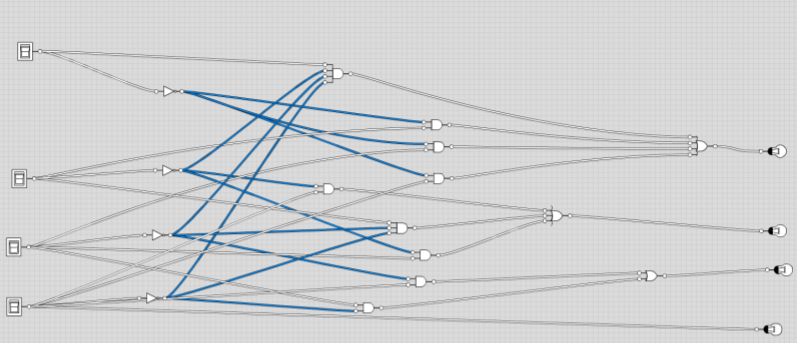
\includegraphics[width=\linewidth]{Ejercicios/CircuitoLogico.png}
	\caption{Circuito logico}
\end{figure}


\chapter*{5 - Sumador BCD}
\section{Objetivo}
  Un sumador BCD posee una funci\'on bastante autoexplicativa, esta es la de tomar 2 valores en expresi\'on binaria y presentar la suma de esta en un formato BCD.
  \section{Implementaci\'ion}
  A la hora de desarrollar el programa se han tenido en cuenta los conceptos de modularizaci\'on y reutilizaci\'on de codigo por lo que este ha comprendido distintas etapas con sus propias funcionalidades. Por lo tanto la implementaci\'on final del codigo ha comprendido distitas estapas las cuales se aboradaran a continuaci\'on.
  \subsection{Adder de 1bit}
  El primer circuito l\'ogico necesario para todas las siguientes implementaciones fue sumador de 1 bit, este tiene la funci\'on de realizar la suma de 2 valores de un bit arrojando como parametros de salida tanto el bit resultante como el bit \emph{carry} generado por estos. este circuito se logra realizando una funci\'on AND a los parametros de entrada, llamese estos \emph{A} y \emph{B}, obteniendo de ese modo el bit de salida \emph{Y} y paralelamente realizando una funcion XOR a los mismos y definiendo de ese modo el valor carry de salida. Este circuito se puede ver representado en el siguiente diagrama:
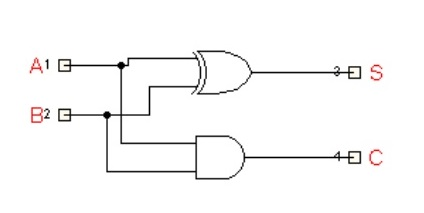
\includegraphics[width=\textwidth]{Ejercicios/adder.jpg}
\subsection{Full-Adder de 1bit}
 Una vez obtenido el Adder se implementa este para lograr el Full-Adder de un bit el cual cumple las mismas funciones basicas con la salvedad que este es capaz de recibir ademas un bit carry como parametro de entrada. Las funciones que cumple el Adder de un bit en el funcionamiento del Full Adder son las siguientes, en primer lugar se tratan los bit de entrara \emph{A} y \emph{B}, estos son aplicados al Adder de ese modo obteniendo un bit de carry que llamaremos \emph{Co1} y una salida \emph{Y1}, lo siguiente sera realizar un Adder con los valores Y1 y el carry de entrada \emph{Cin}, una vez en este punto ya tendremos el bit de salida deasado junto con un segundo bit carry de salida, llamese \emph{Co2}, por lo que resta definir cual sera el bit de carry a la salida del circuito. Este ultimo se obtiene realizando una función OR a los 2 bits carry \emph{Co1} y \emph{Co2}. A continuación se muestra el diagrama del Full-Adder de 1 bit:
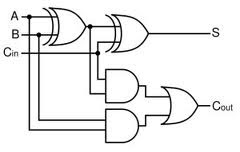
\includegraphics[width=\textwidth]{Ejercicios/full adder.jpg}
\subsection{Full-Adder de 4 bits}
  Contando ya con el Full Adder de 1 bit se escala el funcionamiento de este para lograr realizar la función de suma para valores binarios de 4 bits. Para ello el procedimiento que se realiza es el de tomar de a pares los bits que componen los nibbles con los que se trabaja comenzando por los menos significativos, estos son tratados con el Full Adder (siendo el bit carry de entrada 0) y de aqui se obtiene el bit menos significativo del nibble de salida, por otro lado el bit carry que se obtinene sera el mismo ingresado como el de entrada al Full Adder al que se ingresaran los siguientes bits de los nibbles de entrada. Asi se obtendran los bits de salida yendo del menos significativo al mas significativo y, a su vez, el bit carry de salida producto del ultimo Full Adder de 1 bit implementado sera el que determine si se produjo carry al finalizar la suma.
\\
\subsection{Diseño del Sumador BCD}
  Una vez contando con todas estas herramientas nos disponemos a desarrollar el sumador BCD, para esto el procedimiento a seguir es el siguiente. El suamdor recibira como parametros de entrada 2 nibbles que se llamaran \emph{A} y \emph{B} estos seran ingresados a un bloque Full-Adder de 4 bits, el cual como se sabe devolvera el nibble de salida junto con el bit carry generado, con estos datos se veran si se cumplen alguna de las siguientes condiciones: por un lado si el nibble de salida comprende un numero decimal mayor a 9, o si se ha producido carry en la suma, esto determinara el valor de una señal que actuara como selector de un dispositivo MUX, el cual dependiendo del estado del selector arrojara a la salida un valor decimal de 6, el cual sera el factor de corrección que convierta el valor en expresión binaria a BCD,  o un valor nulo. Por último se tomara el nibble de salida del bloque Adder anterior y el valor a la salida del MUX y se haran pasar estos por un nuevo bloque Full-Adder de 4 bits el cual devolvera un nuevo nibble de salida y el carry de la suma. El criterio que se siguio fue el de devolver el nibble menos significtivo de la suma y un bit carry que indique si el mas significativo comprende un 1 o 0, debido a que la suma de 2 números dara un valor por debajo de 20. Se aclara ademas que la operación se suma de hizo robusta de tal menera que también informara si los parametros de entrada no son validos
\chapter*{6-ALU}
\section{Objetivo}
Implementar una ALU que cumpla con las operaciones basicas 
\textit{SUMA, RESTA, AND, OR, NOT, XOR, CA2, SHFT2}.
\subsection{Criterio e implementaci\'on}
Siguiendo las recomendaciones de la comunidad de Verilog la cual recomienda escribir el codigo de la manera más explicita posible para el compilador.
La ALU tiene como entradas un selector de operaciones de $3 bits$ y dos registros A y B de $4 bits$ cada uno.
Se implementaron las operaciones haciendo uso de las funciones ya aportadas por el lenguaje. Para la selección de operacion se hizo uso de un bloque switch que junto con el bloque @always refresca el estado del programa cada vez que ocurre un cambio en el selector de acción.
Se implemento una CLI en Python con el fin de aumentar la interacción con la misma sin sacrificar su funcionalidad. Esto ha sido realizado con fines experimentales. Notese que esta interfaz no se entromete con el codigo fuente original de Verilog, simplemente lo utiliza.




\end{document}




